\subsection{Legacy Watcher}

The legacy watcher is the standard (for now) watcher system GUI. It is written in OpenGL, wrapped in a creamy Qt shell. 

{\it legacyWatcher} source code can be found in {\tt .\slash src\slash clients\slash legacyWatcher}. The binary produced after building is 
named {\tt watcher}. 

\label{LegacyWatcher}
\begin{figure}[ht]
\centering
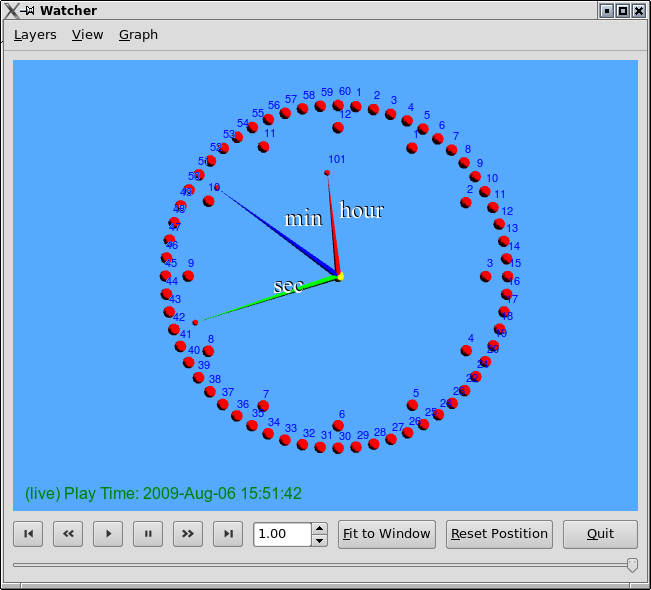
\includegraphics[width=0.8\textwidth]{legWatcherGUI.eps}
\caption{The legacy watcher showing a running instance of showClock.}
\label{fig:LegacyWatcherClock}
\end{figure}

\subsubsection{Configuration}

\begin{itemize}
\item {\tt -h} or {\tt --help}, show a usage message and exit. 
\item {\tt -c configfile}, gives the location of the configuration file. If not given a default one will be created, used, and saved on program exit.
\item {\tt -s {\it float}} or {\tt --speed={\it float}}, specify the event playback speed.
\item {\tt -S {\it int}} or {\tt --seek={\it int}}, specify the offset in milliseconds to start event playback (default: live playback).
\end{itemize}

\subsubsection{Command Line Options}

\begin{itemize}
\item {\tt server}, name or ipaddress of the server to connect to.
\item {\tt service}, name of service (usaully "watcherd") or port number on which the server is listening.
\end{itemize}
